\documentclass{beamer}
\usepackage{beamerthemesplit}
\usepackage{graphicx}
\usepackage{color}
\usepackage{tikz}
\usetikzlibrary{through}
\usepackage{float}
\usepackage{caption}
\usepackage{subcaption}
\usepackage{pgf,pgffor}
\setbeamertemplate{footline}{}


% ============================================================
% Title
% ============================================================

\title{Distributed Graph Coloring}
\subtitle{Based on the Japanese tree frog calling behaviour}
\author[Vajda, Barthel, Godfroid] % (optional, for multiple authors)
{Q.~Vajda \and X.~Barthel \and M.~Godfroid}
\subject{Computer science, Graph, Coloring}
\date{\today}

\begin{document}

\frame{\titlepage}

% ============================================================
\section{Introduction}
% ============================================================

\subsection{Summerize}

\begin{frame} 
\frametitle{Introduction}
  \begin{itemize}
    \item	Graph coloring problem.
    \item	Practical applications.
    \item	Implementation of the FrogSim algorithm.
    \item	Results.
  \end{itemize}
\end{frame}

% ============================================================

\subsection{Graph coloring problem}

\begin{frame} 
\frametitle{Description of the chromatic number problem}
\begin{itemize}
	\item Working on a graph $G$, with a set of node $V$ and a set of edge E.
	\begin{equation*}
	G = (V,E)
	\end{equation*}
	\item A valid k-coloring of a graph is an assignation of a color (within $k$ colors) to each node such that there is not two adjacent nodes with the same color.
	\item Here we want to find a valid coloring using the minimum $k$ needed\footnote{Called the chromatic number of G, $\chi(G)$}.
	\item NP-Hard problem.
\end{itemize}

\end{frame}

% ============================================================
\subsection{Practical applications}

\begin{frame}
\frametitle{Concrete applications}
\begin{itemize}
	\item Frequency assignation for wireless networks.
		\begin{description}
			\item[graph:] a network topology.
			\item[nodes:] the emitters.
			\item[edges:] between the emitters near enough to interfere.
			\item[colors:] the frequencies used by the emitters.
		\end{description}
	\item Jobs scheduling.
		\begin{description}
			\item[graph:] a set of jobs to schedule.
			\item[nodes:] the jobs.
			\item[edges:] the shared resources of the system between two jobs.
			\item[colors:] the time slots.
		\end{description}
\end{itemize}
\end{frame}

% ============================================================
\section{FrogSim algorithm}
% ============================================================

\subsection{Other algorithms}

\begin{frame}
\frametitle{Other algorithm}
This is a NP-hard problem. Then, we use heuristic to solve it.\\
Centralized algorithm:
\begin{itemize}
	\item Genetic algorithm.
	\item DSATUR algorithm.
\end{itemize}

\end{frame}
% ============================================================

\subsection{Initialization}
\begin{frame}
\frametitle{Initialization of the system}
\begin{columns}[t]
	\column{.5\textwidth}
		Each node contains:
		\begin{itemize}
			\item phase value $\theta_i$.
			\item color value $c_i$.
			\item relevance value $r_i$.
			\item a value controlling the amplitude of change $\alpha_i$.
			\item a stack $M_i$ containing the messages sent by the neighbours.
		\end{itemize}
		
	\column{.5\textwidth}
		The system contains:
		\begin{itemize}
			\item a spanning tree.
			\item the root of that tree.
			\item a memorised coloring.
			\item a convergence rate value $\rho$.
		\end{itemize}
	\end{columns}
\end{frame}
% ============================================================

\subsection{Phase 1}

\subsubsection{Event}

\begin{frame}
\frametitle{Event during phase 1 execution}
When an event occurs for a node $i$:
\begin{enumerate}
	\item $\theta_i = \theta_i + \alpha_i \times \sum r_m * inc(\theta_m-\theta_i)$, where:
		\begin{align*}
			inc(x) = 
			\begin{cases}
				x-0.5 & \text{if } x \geq 0 \\
				x+0.5 & \text{if } x < 0
			\end{cases}
		\end{align*}
	\item $c_i = \min \left\lbrace c \in \mathbb{N} | c \neq c_m \forall m \in M_i \right\rbrace$
	\item $m = \left\langle \theta_m, c_m, relevance_m \right\rangle$
	\item $\alpha_i = \frac{\alpha_i}{\rho}$
\end{enumerate}
\end{frame}
% ============================================================

\subsubsection{The desynchronization principle}
\begin{frame}
\begin{figure}[t]
	\centering
	\begin{subfigure}[b]{0.3\textwidth}
		\begin{tikzpicture}
			\pgfmathsetmacro\CA{1.25*cos(296)}
			\pgfmathsetmacro\SA{1.25*sin(296)}

			\pgfmathsetmacro\CB{1.25*cos(310)}
			\pgfmathsetmacro\SB{1.25*sin(310)}

			\pgfmathsetmacro\CC{1.25*cos(151)}
			\pgfmathsetmacro\SC{1.25*sin(151)}

			\pgfmathsetmacro\CD{1.25*cos(93)}
			\pgfmathsetmacro\SD{1.25*sin(93)}
			
			\pgfmathsetmacro\CE{1.25*cos(262)}
			\pgfmathsetmacro\SE{1.25*sin(262)}
			
			\coordinate (a) at (\SA,\CA);
			\coordinate (b) at (\SB,\CB);
			\coordinate (c) at (\SC,\CC);
			\coordinate (d) at (\SD,\CD);
			\coordinate (e) at (\SE,\CE);
			
			\node [draw, circle through={(a),(b)}] at (0,0) {};
			\node [draw, circle, fill=white, minimum size=1mm] at (\SA,\CA) {\tiny{1}};
			\node [draw, circle, fill=white, minimum size=1mm] at (\SB,\CB) {\tiny{2}};
			\node [draw, circle, fill=white, minimum size=1mm] at (\SC,\CC) {\tiny{3}};
			\node [draw, circle, fill=white, minimum size=1mm] at (\SD,\CD) {\tiny{4}};
			\node [draw, circle, fill=white, minimum size=1mm] at (\SE,\CE) {\tiny{5}};
			
			\draw [color=gray] (b) -- (a);
			\draw [color=gray] (b) -- (c);
			\draw [color=gray] (b) -- (d);
			\draw [color=gray] (b) -- (e);
			\draw [color=gray] (a) -- (c);
			\draw [color=gray] (a) -- (d);
			\draw [color=gray] (d) -- (e);
			\draw [color=gray] (c) -- (e);

		\end{tikzpicture}
	\end{subfigure}%
	\begin{subfigure}[b]{0.3\textwidth}
		\begin{tikzpicture}
			\pgfmathsetmacro\CA{1.25*cos(260)}
			\pgfmathsetmacro\SA{1.25*sin(260)}

			\pgfmathsetmacro\CB{1.25*cos(0)}
			\pgfmathsetmacro\SB{1.25*sin(0)}

			\pgfmathsetmacro\CC{1.25*cos(135)}
			\pgfmathsetmacro\SC{1.25*sin(135)}

			\pgfmathsetmacro\CD{1.25*cos(120)}
			\pgfmathsetmacro\SD{1.25*sin(120)}
			
			\pgfmathsetmacro\CE{1.25*cos(249)}
			\pgfmathsetmacro\SE{1.25*sin(249)}
			
			\coordinate (a) at (\SA,\CA);
			\coordinate (b) at (\SB,\CB);
			\coordinate (c) at (\SC,\CC);
			\coordinate (d) at (\SD,\CD);
			\coordinate (e) at (\SE,\CE);
			\node [draw, circle through={(a),(b)}] at (0,0) {};

			\node [draw, circle, fill=white, minimum size=1mm] at (\SA,\CA) {\tiny{1}};
			\node [draw, circle, fill=white, minimum size=1mm] at (\SB,\CB) {\tiny{2}};
			\node [draw, circle, fill=white, minimum size=1mm] at (\SC,\CC) {\tiny{3}};
			\node [draw, circle, fill=white, minimum size=1mm] at (\SD,\CD) {\tiny{4}};
			\node [draw, circle, fill=white, minimum size=1mm] at (\SE,\CE) {\tiny{5}};

			\draw [color=gray] (b) -- (a);
			\draw [color=gray] (b) -- (c);
			\draw [color=gray] (b) -- (d);
			\draw [color=gray] (b) -- (e);
			\draw [color=gray] (a) -- (c);
			\draw [color=gray] (a) -- (d);
			\draw [color=gray] (d) -- (e);
			\draw [color=gray] (c) -- (e);

		\end{tikzpicture}
	\end{subfigure}
	\begin{subfigure}[b]{0.3\textwidth}
		\begin{tikzpicture}
			\pgfmathsetmacro\CB{1.25*cos(10)}
			\pgfmathsetmacro\SB{1.25*sin(10)}

			\pgfmathsetmacro\CD{1.25*cos(112)}
			\pgfmathsetmacro\SD{1.25*sin(112)}
			
			\pgfmathsetmacro\CE{1.25*cos(267)}
			\pgfmathsetmacro\SE{1.25*sin(267)}
			
			\coordinate (b) at (\SB,\CB);
			\coordinate (d) at (\SD,\CD);
			\coordinate (e) at (\SE,\CE);
			\node [draw, circle through={(a),(b)}] at (0,0) {};

			\node [draw, circle, fill=white, minimum size=1mm] at (\SB,\CB) {\tiny{2}};
			\node [draw, circle, fill=white, minimum size=1mm] at (\SD,\CD) {\tiny{3,4}};
			\node [draw, circle, fill=white, minimum size=1mm] at (\SE,\CE) {\tiny{1,5}};

			\draw [color=gray] (b) -- (d);
			\draw [color=gray] (b) -- (e);
			\draw [color=gray] (d) -- (e);
			
		\end{tikzpicture}
	\end{subfigure}\\
	\caption{Example for two oscillators.}\label{fig:Phase_Shift}
\end{figure}
\begin{figure}[b]
	\centering
	\begin{subfigure}[b]{0.35\textwidth}
		\includegraphics[scale=0.25]{Figure/basicGraph.pdf}
	\end{subfigure}%
	\begin{subfigure}[b]{0.35\textwidth}
		\includegraphics[scale=0.25]{Figure/basicGraphColoried.pdf}
	\end{subfigure}
	\caption{Example for two oscillators.}\label{fig:Basic_Coloration}
\end{figure}
\end{frame}

\subsection{Phase 2}

\begin{frame}
\frametitle{Event during phase 2 execution}
An event for a node $i$ during a communication round:\\
\begin{itemize}
	\item For the first round:
		\begin{align*} 
			p_i = 
			\begin{cases}
				r \text{, with } r \text{ random } |\ r \in \mathbb{N} & \text{if } p_i = 1 \\
				0 & \text{if } p_i > 1 
			\end{cases}
		\end{align*}

	\item The other communication rounds:
	\begin{enumerate}
		\item $c_i = \min \left\lbrace c \in \mathbb{N}\ |\ \left(c \neq c_m \land p_m \geq p_i \right) \forall m \in M_i \right\rbrace$
		\item $p_i = \max\lbrace p_m\ |\ m \in M_i\rbrace$
		\item $m = \left\langle c_m, p_m \right\rangle$
	\end{enumerate}
\end{itemize}
\end{frame}
% ============================================================

\section{Results}
% ============================================================

\subsection{Evolution of the coloring through an execution}
\begin{frame}
\begin{overprint}
\foreach \n in {1,...,20}{%
\only<\n>{
	\begin{figure}[h]
		\centering
		\includegraphics[scale=0.2]{Figure/frames/sirs\n.png}
		\caption{Coloration at $round=\n$}
	\end{figure}
}}
\end{overprint}
\end{frame}

% ============================================================
\subsection{Geometric topology}
\begin{frame}
\frametitle{Geometric topology}
\begin{figure}[t]
	\centering
	\begin{subfigure}[h]{0.4\textwidth}
		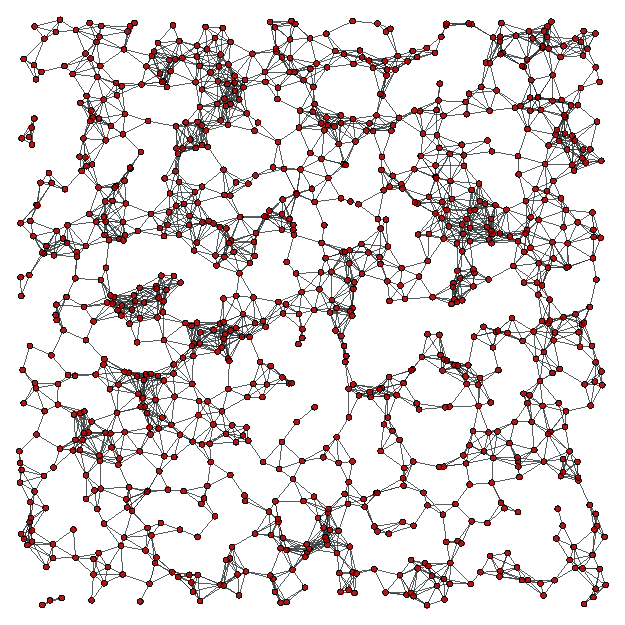
\includegraphics[width=\linewidth]{Figure/geometric.pdf}
		\caption{\footnotesize{Instance of a geometric toplogy of 350 nodes.}}\label{fig:Geo}
	\end{subfigure}%
	\hspace{20pt}
	\begin{subfigure}[h]{0.4\textwidth}
		\includegraphics[width=\linewidth]{Figure/geo-sub_fully_connected.pdf}
		\caption{\footnotesize{$k$-clique of the graph with $k$ maximal.}}\label{fig:CliqueColoration}
	\end{subfigure}
\end{figure}
\end{frame}

\begin{frame}
\frametitle{Geometric topology}
\begin{figure}[b]
	\centering
	\includegraphics[height=0.65\textheight]{Figure/geo-coloried.pdf}
	\caption{Result coloring returned by the FrogSim algorithm.}\label{fig:GeoColoration}
\end{figure}
\end{frame}

\subsubsection{Desynchronization}
\begin{frame}
\begin{figure}[t]
	\centering
	\begin{subfigure}[h]{0.4\textwidth}
		\includegraphics[width=\linewidth]{Figure/phase_avg.pdf}
		\caption{\footnotesize{Average of all the phase of a system.}}\label{fig:Phase_avg}
	\end{subfigure}%
	\hspace{20pt}
	\begin{subfigure}[h]{0.4\textwidth}
		\includegraphics[width=\linewidth]{Figure/dyn_conv.pdf}
		\caption{\footnotesize{Phases of a fully connected graphe of 10 nodes.}}\label{fig:Phases}
	\end{subfigure}
\end{figure}
\begin{figure}[b]
	\centering
	\vspace{-20pt}
	\includegraphics[height=0.35\textheight]{Figure/all_nodes.pdf}
	\caption{Phase value for all the nodes of a system.}\label{fig:CompleteSystem}
\end{figure}

\end{frame}

% ============================================================
\subsection{Grid topology}
\begin{frame}
\frametitle{Grid topology}
\begin{figure}[t]
	\centering
	\begin{subfigure}[h]{0.4\textwidth}
		\includegraphics[width=\linewidth]{Figure/grid.pdf}
		\caption{\footnotesize{Instance of a grid topology $10x10$.}}\label{fig:Grid}
	\end{subfigure}%
	\hspace{20pt}
	\begin{subfigure}[h]{0.4\textwidth}
		\includegraphics[width=\linewidth]{Figure/grid-coloration.pdf}
		\caption{\footnotesize{Result coloring returned by the fromSim.}}\label{fig:GridColoration}
	\end{subfigure}
\end{figure}
\end{frame}

% ============================================================
\section{Conclusion}
% ============================================================

\begin{frame} 
\frametitle{The END}
\begin{center}
	\large{\textbf{Thanks you for listening.}}\\
	Any questions ?
	
\end{center}

\end{frame}


% ============================================================

\end{document}
